\documentclass[11pt]{article}
\usepackage[paper=letterpaper, left=1in, right=1in, top=1in, bottom=1in]
           {geometry}
\usepackage[parfill]{parskip}
\usepackage{amsmath}
\usepackage{graphicx}
\usepackage{fancyvrb}
\usepackage{upquote}

\begin{document}
\thispagestyle{empty}

\begin{center}
{\large CS 310}\\
Assignment 131
\end{center}

\begin{flushright}
William Briggs
\end{flushright}

\textbf{Problem 1.} Use the definitions to prove or disprove the
statement $n(n + 1)/2 \in \Omega(n)$, and illustrate this graphically.

\textit{Answer:} The definition requires us to find $c$ and $n_0$ so that
\[
\frac{n(n + 1)}{2} \geq cn \text{ when } n \geq n_0
\]

We can simplify this to:
\[
\frac{n + 1}{2} \geq c
\]

And we know that $c$ must be equal to or less than the limit of this function.
\[
\lim_{n \to \infty}\frac{n + 1}{2} = \infty
\]

Since must be $c \leq \infty$, let $c = 2$. Thus $n_0 = 3$, and
\[
\frac{n(n + 1)}{2} \geq 2n \text{ when } n \geq 3
\]

Therefore $n(n + 1)/2 \in \Omega(n)$ by the definition of Big-Omega. QED.

This is graphically illustrated by the following plot that shows
$n(n + 1)/2$ along with the standard function $n$ and the function $n$ scaled by
the constant coefficient $c = 2$.

% change 0.7 depending on the size of your graphic
% make sure the image fits on the page and is legible, without
% noticeable pixellation
\begin{center}
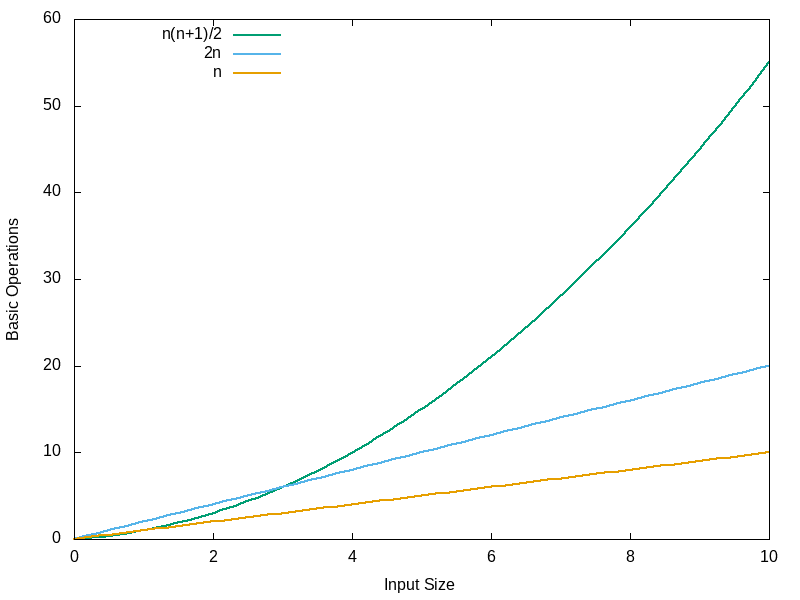
\includegraphics[width=0.7\textwidth]{problem_1.png}
\end{center} 

\textbf{Problem 2.} Using the definitions, either prove the following
assertion, or disprove it with a specific counterexample:
\[
\text{if } t(n) \in O(g(n)) \text{ then } g(n) \in \Omega(t(n))
\]
\textit{Answer:} Assume $t(n) \in O(g(n))$, therefore there is a constant $c_1 > 0$, and $n_0$ such that $n > n_0$. Thus,
\[
t(n) \leq c_1 * g(n) \text{ when } n > n_0
\]
Therefore,
\[
\frac{1}{c_1} * t(n) \leq g(n) \text{ when } n > n_0
\]
So if we let $c_2 = \frac{1}{c_1}$, where $c_2$ is a constant $c_2 > 0$. We can similarly write:
\[
g(n) \geq c_2 * t(n) \text{ when } n > n_0
\]
This is the definition of Big Omega. We can conclude then that: if $t(n) \in O(g(n))$ then $g(n) \in \Omega(t(n))$. QED.

\newpage
\textbf{Problem 3.} For the following algorithm, explain what it
computes, state what the input size for analysis is, state what basic
operations should be counted for analyzing it, state exactly how many
operations are executed as a function of the input size, and state the
efficiency class to which it belongs.


\begin{Verbatim}[numbers=left,xleftmargin=5mm]
void foo(vector & array)
{
  size_t n {array.size()};
  for (size_t select_index {0}; select_index < n - 1; select_index++)
  {
    auto smallest_value {array.at(select_index)};
    auto smallest_index {select_index};
    for (auto compare_index {select_index + 1}; compare_index < n;
         compare_index++)
    {
      if (array.at(compare_index) < smallest_value)
      {
        smallest_value = array.at(compare_index);
        smallest_index = compare_index;
      }
    }
    swap(array.at(smallest_index), array.at(select_index));
  }
}
\end{Verbatim}

\textit{Answer:} This algorithm sorts an array from least to greatest value. The input size for this algorithm is equal to the size of the array, determined at Line 3. For counting the number of operations, we count every assignment (i.e. Line 6) and logical operator (i.e. Line 11), being careful to check each statement for multiples of either (Line 4). Specifically look at line 8, this For Loop executes $n(n-1)/2$ times, which is the summation of numbers from $1$ to $n-1$. Therefore, I found the operations to follow this function:
\[
T(n) = 2 + 2n + 7(n-1) + \frac{3n(n-1)}{2}
\]
\[
T(n) = \frac{3}{2}n^{2} + \frac{15}{2}n - 5 
\]
\[
  T(n) \in O(n^{2})
\]
\[
  T(n) \in \Omega(n^{2})
\]

or equivalently,

\[
T(n) \in \Theta(n^{2})
\]

\newpage
\textbf{Problem 4.} Write a C++ program that implements the algorithm
in problem 3, counts the number of basic operations, and outputs the
input size and the count of basic operations to the cerr stream. Run
this program many times with many different inputs and capture the
results.

Use a plot of input size vs.\ basic operations, along with one or more
standard functions properly scaled, to illustrate your analysis, and
include this in your document.

\textit{Answer:} See the attached program. When it is run with the
command

\begin{Verbatim}
for n in `seq 10 10 1000`
do
    ./assignment_131 $n
done > /dev/null 2> results.dat
\end{Verbatim}

and the resulting data file is plotted with gnuplot, the following is
produced. Also plotted on the same axis are the scaled standard
functions $n^2$ and $5n^2$ which shows that the algorithm runs between the two, therefore $f(n) \in \Theta(n^{2})$

\begin{center}
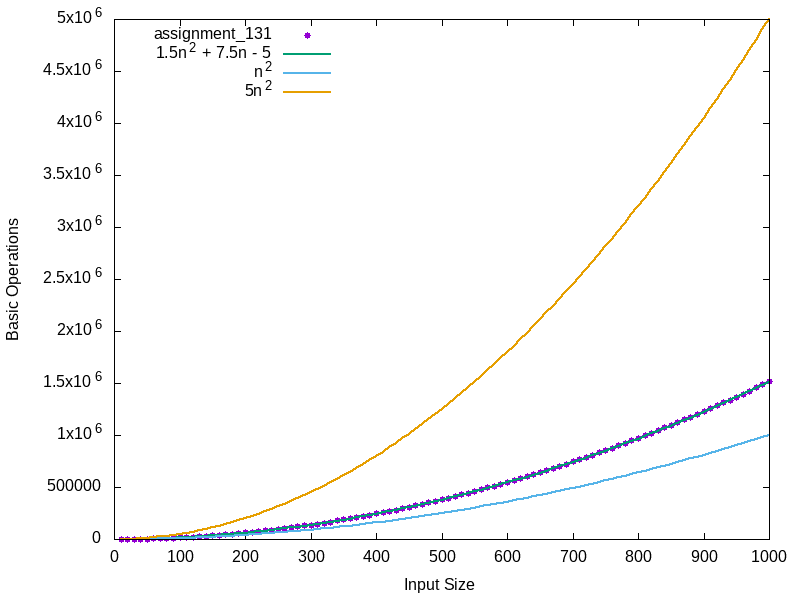
\includegraphics[width=0.7\textwidth]{problem_4.png}
\end{center} 

\end{document}